\documentclass[t,aspectratio=169]{beamer} % 使用16:9宽高比
\usetheme{Madrid} % 选择Madrid主题
\usecolortheme{default} % 使用默认颜色主题

% 设置字体
\usepackage[UTF8]{ctex}
\usefonttheme{structurebold} % 加粗结构字体

% 数学包
\usepackage{amsmath, amssymb, bm}
\usepackage{url}

% 图形包 (如果需要插入图片)
\usepackage{graphicx}
% \graphicspath{{./images/}} % 假设图片放在images文件夹

% 算法包
\usepackage{algorithm}
\usepackage{algpseudocode}
\usepackage{xcolor}
\renewcommand{\algorithmiccomment}[1]{\hfill\texttt{\textcolor{violet}{// #1}}}
\algnewcommand\algorithmicinput{\textbf{Input:}}
\algnewcommand\algorithmicoutput{\textbf{Output:}}
\algnewcommand\Input{\item[\algorithmicinput]}
\algnewcommand\Output{\item[\algorithmicoutput]}

% 标题页信息
\title[7.3.收敛性]{第7章：梯度下降}
\subtitle{第3节：收敛性 (Convergence)}
\author{《深度学习基础》课程小组}
% \institute{上海立信会计金融学院}
\date{\today}

\begin{document}

% 标题页
\frame{\titlepage}

% 目录页
\begin{frame}
    \frametitle{目录}
    \tableofcontents
\end{frame}

% ============================================================
% 第一部分：学习率与收敛问题
% ============================================================
\section{学习率与收敛问题}

\begin{frame}
    \frametitle{1. 学习率的选择与“山谷”问题}
    \begin{itemize}
        \item 应用梯度下降时，需要选择\alert{学习率 $\eta$}。
        \item 考虑误差曲面的“山谷”形状（图 7.3）：曲率随方向显著变化。
        \item 在大多数点上，局部梯度\alert{并不直接指向极小值}。
        \item 直观上增大 $\eta$ 应该加快收敛。
        \item 但实际上：每一步在\alert{山谷两侧来回振荡}。
        \item 若 $\eta$ 太大，振荡会\alert{发散}。
        \item 为避免发散，$\eta$ 必须足够小 $\Rightarrow$ 沿山谷方向进展\alert{非常缓慢}。
    \end{itemize}
\end{frame}

\begin{frame}
    \frametitle{1.1 固定步长梯度下降示意图}
    \begin{figure}
        \centering
        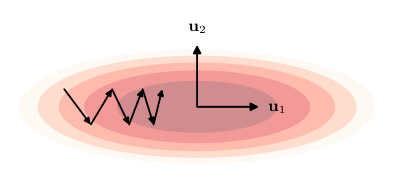
\includegraphics[width=0.4\textwidth]{figure7-3.png}
        \caption{误差曲面呈长山谷形状，梯度下降在两侧振荡，沿山谷方向进展缓慢。}
    \end{figure}
    \begin{itemize}
        \item $u_1$ 和 $u_2$ 是海森矩阵的特征向量。
        \item 相邻步骤在谷壁之间振荡。
    \end{itemize}
\end{frame}

% ============================================================
% 第二部分：二次近似分析
% ============================================================
\section{二次近似分析}

\begin{frame}
    \frametitle{2. 极小值附近的二次近似分析}
    在极小值附近，由 (7.7)(7.8)(7.10)：
    \begin{equation}
    \nabla E = \sum_i \alpha_i \lambda_i \mathbf{u}_i
    \tag{7.24}
    \end{equation}
    权重变化：
    \begin{equation}
    \Delta \mathbf{w} = \sum_i \Delta \alpha_i \mathbf{u}_i
    \tag{7.25}
    \end{equation}
    结合梯度下降公式 (7.16) 和正交性 (7.9)：
    \begin{equation}
    \Delta \alpha_i = -\eta \lambda_i \alpha_i
    \tag{7.26}
    \end{equation}
    \begin{equation}
    \alpha_i^{\mathrm{new}} = (1 - \eta \lambda_i) \alpha_i^{\mathrm{old}}
    \tag{7.27}
    \end{equation}
    $\alpha_i$ 可解释为\alert{沿 $\mathbf{u}_i$ 方向到极小值的距离}。
\end{frame}

\begin{frame}
    \frametitle{2.1 收敛条件与线性收敛}
    经过 $T$ 步后：
    \begin{equation}
    \alpha_i^{(T)} = (1 - \eta \lambda_i)^T \alpha_i^{(0)}
    \tag{7.29}
    \end{equation}
    \begin{itemize}
        \item 若 $|1 - \eta \lambda_i| < 1$，则 $T \to \infty$ 时 $\alpha_i \to 0$，即 $\mathbf{w} \to \mathbf{w}^*$。
        \item 梯度下降在极小值附近呈\alert{线性收敛}。
        \item 收敛要求所有 $\lambda_i > 0$（驻点确实是极小值）。
        \item 增大 $\eta$ 可使 $(1 - \eta \lambda_i)$ 更小，加快收敛。
        \item 但必须保证 $|1 - \eta \lambda_i| < 1$，否则 $\alpha_i$ 发散。
        \item 限制：\alert{$\eta < 2 / \lambda_{\max}$}。
    \end{itemize}
\end{frame}

\begin{frame}
    \frametitle{2.2 条件数与收敛速度}
    \begin{itemize}
        \item 收敛速度由\alert{最小特征值}主导。
        \item 取 $\eta$ 为最大允许值时，沿最小特征值方向的收敛由下式控制：
        \begin{equation}
        \left(1 - \frac{2 \lambda_{\min}}{\lambda_{\max}}\right)
        \tag{7.30}
        \end{equation}
        \item $\lambda_{\min} / \lambda_{\max}$ 的倒数称为海森矩阵的\alert{条件数 (condition number)}。
        \item 若该比值很小（椭圆高度拉长），则收敛\alert{极其缓慢}。
    \end{itemize}
\end{frame}

% ============================================================
% 第三部分：动量
% ============================================================
\section{动量}

\begin{frame}
    \frametitle{3. 动量 (Momentum)}
    \begin{itemize}
        \item 解决特征值差异大问题的简单技术：在梯度下降中加入\alert{动量项}。
        \item 效果：为权重空间中的运动增加\alert{惯性}，平滑振荡。
        \item 修改后的公式：
        \begin{equation}
        \Delta \mathbf{w}^{(\tau-1)} = -\eta \nabla E\left(\mathbf{w}^{(\tau-1)}\right) + \mu \Delta \mathbf{w}^{(\tau-2)}
        \tag{7.31}
        \end{equation}
        \item $\mu$ 称为\alert{动量参数}。
    \end{itemize}
\end{frame}

\begin{frame}
    \frametitle{3.1 低曲率区域：有效学习率增大}
    在低曲率区域（图 7.4），假设梯度不变，迭代求和：
    \begin{align}
    \Delta \mathbf{w} &= -\eta \nabla E \{1 + \mu + \mu^2 + \ldots \} \nonumber \\
    &= -\frac{\eta}{1 - \mu} \nabla E
    \tag{7.32}
    \end{align}
    \begin{itemize}
        \item 动量项的效果：\alert{有效学习率从 $\eta$ 增大到 $\eta/(1-\mu)$}。
        \item 典型值 $\mu = 0.9$ $\Rightarrow$ 有效学习率增大约 10 倍。
    \end{itemize}
\end{frame}

\begin{frame}
    \frametitle{3.2 高曲率区域：抑制振荡}
    \begin{itemize}
        \item 在高曲率区域（图 7.5），梯度下降呈\alert{振荡}状态。
        \item 动量项的连续贡献\alert{相互抵消}，有效学习率接近 $\eta$。
        \item 结论：动量项可以\alert{加速收敛而不引起发散振荡}（图 7.6）。
    \end{itemize}
    \begin{figure}
        \centering
        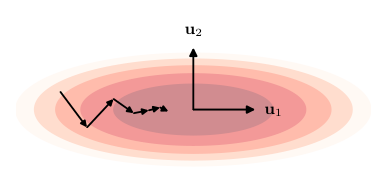
\includegraphics[width=0.3\textwidth]{figure7-6.png}
        \caption{添加动量项后沿山谷方向进展更快。}
    \end{figure}
\end{frame}

\begin{frame}[allowframebreaks]
    \frametitle{3.3 带动量的 SGD 算法}
    \begin{itemize}
        \item 引入第二个参数 $\mu$，范围 $0 \leqslant \mu \leqslant 1$，典型值 $\mu = 0.9$。
    \end{itemize}
    \begin{algorithm}[H]
    \caption{Stochastic gradient descent with momentum}
    \begin{algorithmic}
    \Input Training set $\{1,\dots,N\}$; batch size $B$; error $E_{n:n+B-1}(\mathbf{w})$; $\eta$; $\mu$; initial $\mathbf{w}$
    \Output Final weight vector $\mathbf{w}$
    \State $n \leftarrow 1$; $\Delta\mathbf{w} \leftarrow 0$
    \Repeat
      \State $\Delta \mathbf{w} \leftarrow -\eta \nabla E_{n:n+B-1}(\mathbf{w}) + \mu\Delta \mathbf{w}$ \Comment{带动量更新}
      \State $\mathbf{w}\leftarrow \mathbf{w} + \Delta \mathbf{w}$ \Comment{更新权重}
      \State $n \leftarrow n + B$
      \If{$n + B > N$}
        \State shuffle data; $n \gets 1$
      \EndIf
    \Until{convergence}
    \State \textbf{return} $\mathbf{w}$
    \end{algorithmic}
    \end{algorithm}
\end{frame}

\begin{frame}
    \frametitle{3.4 Nesterov 动量}
    \begin{itemize}
        \item 改变计算顺序：先根据上一步动量走一步，再在新位置计算梯度。
        \begin{equation}
        \Delta \mathbf{w}^{(\tau-1)} = -\eta \nabla E\left(\mathbf{w}^{(\tau-1)} + \mu \Delta \mathbf{w}^{(\tau-2)}\right) + \mu \Delta \mathbf{w}^{(\tau-2)}
        \tag{7.34}
        \end{equation}
        \item 对\alert{批量梯度下降}可改善收敛速度。
        \item 对\alert{随机梯度下降}效果可能较弱。
    \end{itemize}
\end{frame}

% ============================================================
% 第四部分：学习率调度
% ============================================================
\section{学习率调度}

\begin{frame}
    \frametitle{4. 学习率调度 (Learning Rate Schedule)}
    \begin{itemize}
        \item $\eta$ 太小 $\rightarrow$ 学习慢；$\eta$ 太大 $\rightarrow$ 不稳定。
        \item 最佳实践：\alert{训练初期用较大 $\eta$，随时间减小}。
        \begin{equation}
        \mathbf{w}^{(\tau)} = \mathbf{w}^{(\tau-1)} - \eta^{(\tau-1)} \nabla E_n(\mathbf{w}^{(\tau-1)})
        \tag{7.35}
        \end{equation}
        \item 常见调度方式：
        \begin{align}
        \eta^{(\tau)} &= \left(1 - \tau/K\right) \eta^{(0)} + (\tau/K) \eta^{(K)} \tag{7.36} \\
        \eta^{(\tau)} &= \eta^{(0)} \left(1 + \tau/s\right)^c \tag{7.37} \\
        \eta^{(\tau)} &= \eta^{(0)} c^{\tau/s} \tag{7.38}
        \end{align}
        \item 超参数 $\eta^{(0)}, \eta^{(K)}, K, S, c$ 需\alert{经验性选择}。
        \item 建议监控\alert{学习曲线}，确保误差以合适速率下降。
    \end{itemize}
\end{frame}

% ============================================================
% 第五部分：RMSProp 与 Adam
% ============================================================
\section{RMSProp 与 Adam}

\begin{frame}
    \frametitle{5. 自适应学习率算法}
    \begin{itemize}
        \item 最优学习率取决于误差曲面的\alert{局部曲率}。
        \item 曲率随参数空间方向变化。
        \item 动机：为每个参数使用\alert{不同的学习率}，自动调整。
        \item 注意：这种直觉在\alert{局部对角海森矩阵}时成立，实际中不常见，但这些算法仍然有效且广泛使用。
    \end{itemize}
\end{frame}

\begin{frame}
    \frametitle{5.1 AdaGrad}
    \begin{itemize}
        \item 核心思想：用\alert{梯度平方的累积和}来减小每个参数的学习率。
        \item 高曲率参数的学习率减小最快。
        \begin{align}
        r_i^{(\tau)} &= r_i^{(\tau-1)} + \left(\frac{\partial E(\mathbf{w})}{\partial w_i}\right)^2 \tag{7.39} \\
        w_i^{(\tau)} &= w_i^{(\tau-1)} - \frac{\eta}{\sqrt{r_i^{\tau}} + \delta} \left(\frac{\partial E(\mathbf{w})}{\partial w_i}\right) \tag{7.40}
        \end{align}
        \item $\delta \approx 10^{-8}$ 保证数值稳定性。
        \item \textbf{问题}：从训练开始就累积平方梯度，后期更新量过小，训练过慢。
    \end{itemize}
\end{frame}

\begin{frame}
    \frametitle{5.2 RMSProp}
    \begin{itemize}
        \item 将 AdaGrad 的\alert{平方梯度和}替换为\alert{指数加权平均}。
        \begin{align}
        r_i^{(\tau)} &= \beta r_i^{(\tau-1)} + (1 - \beta) \left(\frac{\partial E(\mathbf{w})}{\partial w_i}\right)^2 \tag{7.41} \\
        w_i^{(\tau)} &= w_i^{(\tau-1)} - \frac{\eta}{\sqrt{r_i^{\tau}} + \delta} \left(\frac{\partial E(\mathbf{w})}{\partial w_i}\right) \tag{7.42}
        \end{align}
        \item 典型值 $\beta = 0.9$。
    \end{itemize}
\end{frame}

\begin{frame}[allowframebreaks]
    \frametitle{5.3 Adam：RMSProp + 动量}
    \begin{itemize}
        \item 名称来自\alert{adaptive moments}。
        \item 为每个参数\alert{分别存储动量}，对梯度和平方梯度都使用指数加权移动平均。
        \begin{align}
        s_i^{(\tau)} &= \beta_1 s_i^{(\tau-1)} + (1 - \beta_1) \left(\frac{\partial E(\mathbf{w})}{\partial w_i}\right) \tag{7.43} \\
        r_i^{(\tau)} &= \beta_2 r_i^{(\tau-1)} + (1 - \beta_2) \left(\frac{\partial E(\mathbf{w})}{\partial w_i}\right)^2 \tag{7.44} \\
        \widehat{s}_i^{(\tau)} &= \frac{s_i^{(\tau)}}{1 - \beta_1^\tau} \tag{7.45} \\
        \widehat{r}_i^{(\tau)} &= \frac{r_i^{(\tau)}}{1 - \beta_2^\tau} \tag{7.46} \\
        w_i^{(\tau)} &= w_i^{(\tau-1)} - \eta \frac{\widehat{s}_i^{\tau}}{\sqrt{\widehat{r}_i^{\tau}} + \delta} \tag{7.47}
        \end{align}
        \item 偏差修正：$1/(1-\beta_1^\tau)$ 和 $1/(1-\beta_2^\tau)$ 修正零初始化带来的偏差。
        \item 典型值：$\beta_1 = 0.9$，$\beta_2 = 0.99$。
        \item Adam 是深度学习中最广泛采用的优化算法。
    \end{itemize}
\end{frame}

\begin{frame}[shrink=28]
    \frametitle{5.4 Adam 算法伪代码}
    \footnotesize
    \begin{algorithm}[H]
    \caption{Adam optimization}
    \begin{algorithmic}
    \Input $\{1,\dots,N\}$; $B$; $E_{n:n+B-1}(\mathbf{w})$; $\eta$; $\beta_1, \beta_2$; $\delta$
    \Output Final weight vector $\mathbf{w}$
    \State $n \leftarrow 1$; $s \leftarrow 0$; $r \leftarrow 0$
    \Repeat
      \State 随机选择一个小批量
      \State $g=-\nabla E_{n:n+B-1}(w)$
      \State $s\leftarrow \beta_1s + (1-\beta_1)g$
      \State $r\leftarrow \beta_2r + (1-\beta_2)g\odot g$
      \State $\hat{s}\leftarrow s/(1-\beta_1^\tau)$
      \State $\hat{r}\leftarrow r/(1-\beta_2^\tau)$
      \State $\Delta \mathbf{w} \leftarrow -\eta \frac{\hat{s}}{\sqrt{\hat{r}}+\delta}$
      \State $\mathbf{w}\leftarrow \mathbf{w} + \Delta \mathbf{w}$
      \State $n \leftarrow n + B$
      \If{$n + B > N$}
        \State shuffle data; $n \gets 1$
      \EndIf
    \Until{convergence}
    \State \textbf{return} $\mathbf{w}$
    \end{algorithmic}
    \end{algorithm}
\end{frame}

% ============================================================
% 第六部分：总结
% ============================================================
\section{总结}

\begin{frame}
    \frametitle{6. 本节总结}
    \begin{itemize}
        \item \alert{学习率 $\eta$} 的选择至关重要：太大导致振荡发散，太小收敛缓慢。
        \item \alert{二次近似分析}：收敛速度由条件数 $\lambda_{\max}/\lambda_{\min}$ 决定。
        \item \alert{动量}：增加惯性，低曲率区域增大有效学习率，高曲率区域抑制振荡。
        \item \alert{Nesterov 动量}：改变计算顺序，对批量梯度下降更有效。
        \item \alert{学习率调度}：训练初期用大 $\eta$，随时间减小（线性、幂律、指数衰减）。
        \item \alert{自适应学习率算法}：
        \begin{itemize}
            \item \textbf{AdaGrad}：累积平方梯度，后期更新过小。
            \item \textbf{RMSProp}：指数加权平均，解决 AdaGrad 后期过慢问题。
            \item \textbf{Adam}：RMSProp + 动量 + 偏差修正，最广泛使用。
        \end{itemize}
    \end{itemize}
\end{frame}

% ============================================================
% 第七部分：参考文献
% ============================================================
\section{参考文献}

\begin{frame}
    \frametitle{7. 参考文献}
    \begin{itemize}
        \item 教材：Bishop, C. M. \& Bishop, H. (2023). Deep Learning Foundations and Concepts. Springer Nature Switzerland AG.
        \item Nesterov, Y. (2004). Introductory Lectures on Convex Optimization.
        \item Duchi, J., Hazan, E., \& Singer, Y. (2011). Adaptive subgradient methods for online learning and stochastic optimization.
        \item Hinton, G. (2012). Lecture 6.5 - RMSProp, COURSERA: Neural Networks for Machine Learning.
        \item Kingma, D. P. \& Ba, J. (2014). Adam: A method for stochastic optimization.
    \end{itemize}
\end{frame}

\end{document}